\chapter{Project Scheduling}
\begin{spacing}{1}
\setlength{\parskip}{0.3in}
\graphicspath{{./Chapter5/}}

\section{Introduction}
Project scheduling is structured listing of tasks, resources and duration  in a time sequenced manner so that the progress can be tracked and the project can be completed on time. Effective project schedule is a critical component of successful time management.
Schedule not only defines the start and end time of each activity or task, it also defines the dependencies among the tasks and the sequence of dependent tasks. A project schedule is created on the early planning phase of the project life cycle and is crucial in the project plan, where the schedule plan, schedule baseline, deliverable and requirements are identified. The project schedule is the guideline to the developer team throughout the execution phase. During the execution phase, the schedule baseline is compared against the actual progress and further modifications are added to the plan. Project scheduling is an iterative process.

\subsection{Scheduling Objectives}
A project schedule is a document that involves all the efforts needed to complete the project on time. It is also not possible to make an effective resource and cost management without a full and accurate work schedule. An effective project schedule provides a better resource and time management scheme and finds a trade off among its primary and secondary objectives.

\begin{itemize}
	\item \textbf{Primary Objectives}
	\begin{enumerate}
		\item \textbf{Best time} \newline Project schedule answers when an activity should start, how long it can take to complete and the deadline to finish the activity. 
		\item \textbf{Least cost} \newline Project schedule defines the what resources are associated with each activity and answers the lowest possible costs to complete each activity in the project.
		\item \textbf{Least risk} \newline Project schedule defines the slack and float available with each activity and dependencies among the activities to maintain.  
	\end{enumerate}
	\item \textbf{Secondary Objectives}
	\begin{enumerate}
		\item \textbf{Propose and evaluate different schedule alternatives} \newline Analyze different sequences of tasks and different schedule for their dependencies.
		\item \textbf{Make an effective use of resources} \newline Schedule the tasks in an cost effective manner so that no resources remain idle for a long period of time.
		\item \textbf{Reduce communication overhead among resources} \newline Project schedule organize the tasks in effective manner so that the resources are well distributed and available to all the components.
	\end{enumerate}
\end{itemize}

\section{Schedule Techniques}
Highly accurate estimation of duration of project tasks is the key concept to create a realistic project schedule. To make accurate estimations, project managers need to discuss with different stakeholders, review their perspectives on the tasks difficulty and possible duration, analyze previous projects and historic data. Alongside project managers follow different scheduling techniques to increase accuracy of their estimations of time and costs. 
Among different scheduling techniques, \textbf{Network Diagrams} uses to graphically represent the tasks of the project and their relationships. \textbf{CPM} and \textbf{PERT} are widely used network diagrams. The \textbf{CPM or Critical Path Method} is an equation that shows the possible longest timeline of the project. The \textbf{PERT or Program Evaluation and Review Technique} is used to visualize the flow of tasks for better estimations and also includes the dependencies.
 A \textbf{Work Breakdown Structure or WBS} is a graphical representation of decomposed tasks and deliverable of the final project. WBS becomes input to many other techniques, specially in the scheduling process. All the steps of the project are outlined in the organizational chart of a work breakdown structure.
 Another popular schedule technique is \textbf{Bar charts}. \textbf{Milestone Charts} is used to graphically represents the tasks in a temporal sequence, the bar length is directly proportional to the duration of that tasks. Another widely used technique is \textbf{Gantt Chart}. Gantt chart is also visualize the temporal sequence of tasks as milestone chart but gantt chart also shows the groups and subgroups of the tasks, dependencies among the tasks and can also shows the progress of each tasks. Gantt chart gives a more details view of the tasks sequence in temporal order.
 
 \subsection{Work Breakdown Structure}
 A work breakdown structure or WBS is visual, structured and hierarchical deconstruction of a project. WBS allows the team to work backward from the final deliverable of a project and identify all the activities needed to achieve a successful product. WBS takes a complex and large project and break down the project scope into more manageable pieces to make it easier to plan, schedule and deliver. WBS is the first step in the project scheduling process and provide the input for further estimation and scheduling techniques. A well structured WBS is created with several key components and some major components are as following:
 \begin{itemize}
 	\item \textbf{WBS Dictionary} \newline
 	A document that defines various elements of the WBS. It helps the team and stakeholders to understand the phases and deliverables.
 	\item \textbf{Task Number and Description} \newline Each task is assigned against a number to easily identify and refer the task in later processes. A description is the detail statement about the task.
 	\item \textbf{Task Dependency} \newline Some tasks have dependencies on other tasks as the dependent task have to wait until some other tasks have been completed. WBS defines the dependencies of each task(if any) in a well mannered way.
 	\item \textbf{Estimated Time Duration} \newline WBS tracks the estimated duration of each task, the start and end date of the tasks so that the tasks can be completed in time.
 	\item \textbf{Task Status} \newline WBS keeps record of the status of each task so the overall work progress can be measured. It is an iterative process and maintained throughout the execution phase.
 \end{itemize} 

As the proposed new system for the AKASH DTH is decomposed in a well structured WBS with each tasks number, description, duration and dependencies. This document works as the map for the project workflows and goals and further used in the CPM, PERT and Gantt Chart techniques. \newline
Time duration of each task is estimated using the top-down approach. The historic data gathered from their previous system's management was a key resource for the estimation and also expert judgment was asked from the previous team before planning the WBS. The dependencies were listed with additional care as the breakdown of the complex project scheduling highly affects from the internal dependencies among the component tasks. WBS was reviewed and the estimations were adjusted by Akash DTH team members.

\begin{table}[h!]
\begin{center}
	\begin{tabular}{| p{1cm}|p{7cm}|p{2cm}|p{3cm} |}
		\hline
		Task ID & Task Description & Est. Duration & Dependencies \\
		\hline
		A & Analysis new proposed data models and functionalities & 14 days & -- \\
		\hline
		B & Designing UI & 21 days & A \\
		\hline
		C & Creating new database tables in a isolated environment & 21 days & A \\
		\hline
		D & Testing new database models integrity and relationships & 15 days & C \\
		\hline
		E & Coding new permission scheme & 15 days & C \\
		\hline
		F & Coding new customer service module & 15 days & C \\
		\hline
		G & Coding new custom package creation and alteration scheme & 15 days & C \\
		\hline
		H & Integrating UI with back-end API endpoints & 28 days & J \\
		\hline
		I & Migrating new database models to production database system & 14 days & D \\
		\hline
		J & Testing back-end API endpoints & 21 days & I, E, F, G \\
		\hline
		K & Testing final UI & 14 days & H \\
		\hline
		L & Testing security features & 21 days & K \\
		\hline    
	\end{tabular}
\end{center}
\caption{WBS chart for proposed system of Akash DTH }
\label{chart:WBS}
\end{table}
  
\section{Network Diagrams}
Network diagrams is a graph like visual representation of the tasks in the WBS chart with the internal relationships and dependencies among the tasks. Network diagrams is a vital tool for the project scheduling and further measuring the work progress. Both the \textbf{CPM} and \textbf{PERT} techniques uses the network diagram technique for project scheduling. Two common methods to represent network diagram are \textbf{AON} or Activity On Node and \textbf{AOA} or Activity On Arrow. For scheduling the proposed system improvement for Akash DTH, we used both AON and AOA graph representations.

\paragraph{Activity On Arrow(AOA) Format}
On activities on arrow or AOA graph format, circles represent the events like start and end of a connected task, and lines represent the tasks. Time goes the direction of the arrow, generally from left to right. Duration and description of a task can be added in the label of the respective line. AOA method is also generally known as \textbf{Arrow Diagramming Method(ADM)}. AOA network graph for the  WBS listed in the table \ref{chart:WBS} is shown in Figure \ref{fig:aoa}.

\begin{figure}[H]
	\centering
	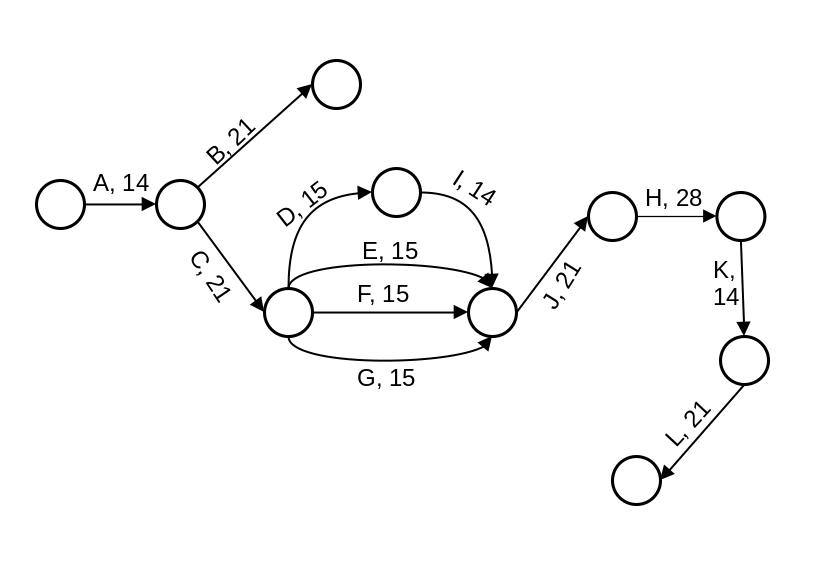
\includegraphics[width=0.8\textwidth]{AOA}
	\caption{AOA network graph}
	\label{fig:aoa}
\end{figure} 

\paragraph{Activities On Node(AON) Format}
On activities on node or AON network, nodes are either presented with a circle or rectangle, task duration, description, start, end dates are presented also in the nodes and arrows represent the dependencies among the connected nodes ar tasks. AON is also popularly referred as \textbf{Precedence Diagramming Method (PDM)}.A simple AON network graph for the WBS in the table \ref{chart:WBS} is shown in Figure \ref{fig:aon}.

\begin{figure}[H]
	\centering
	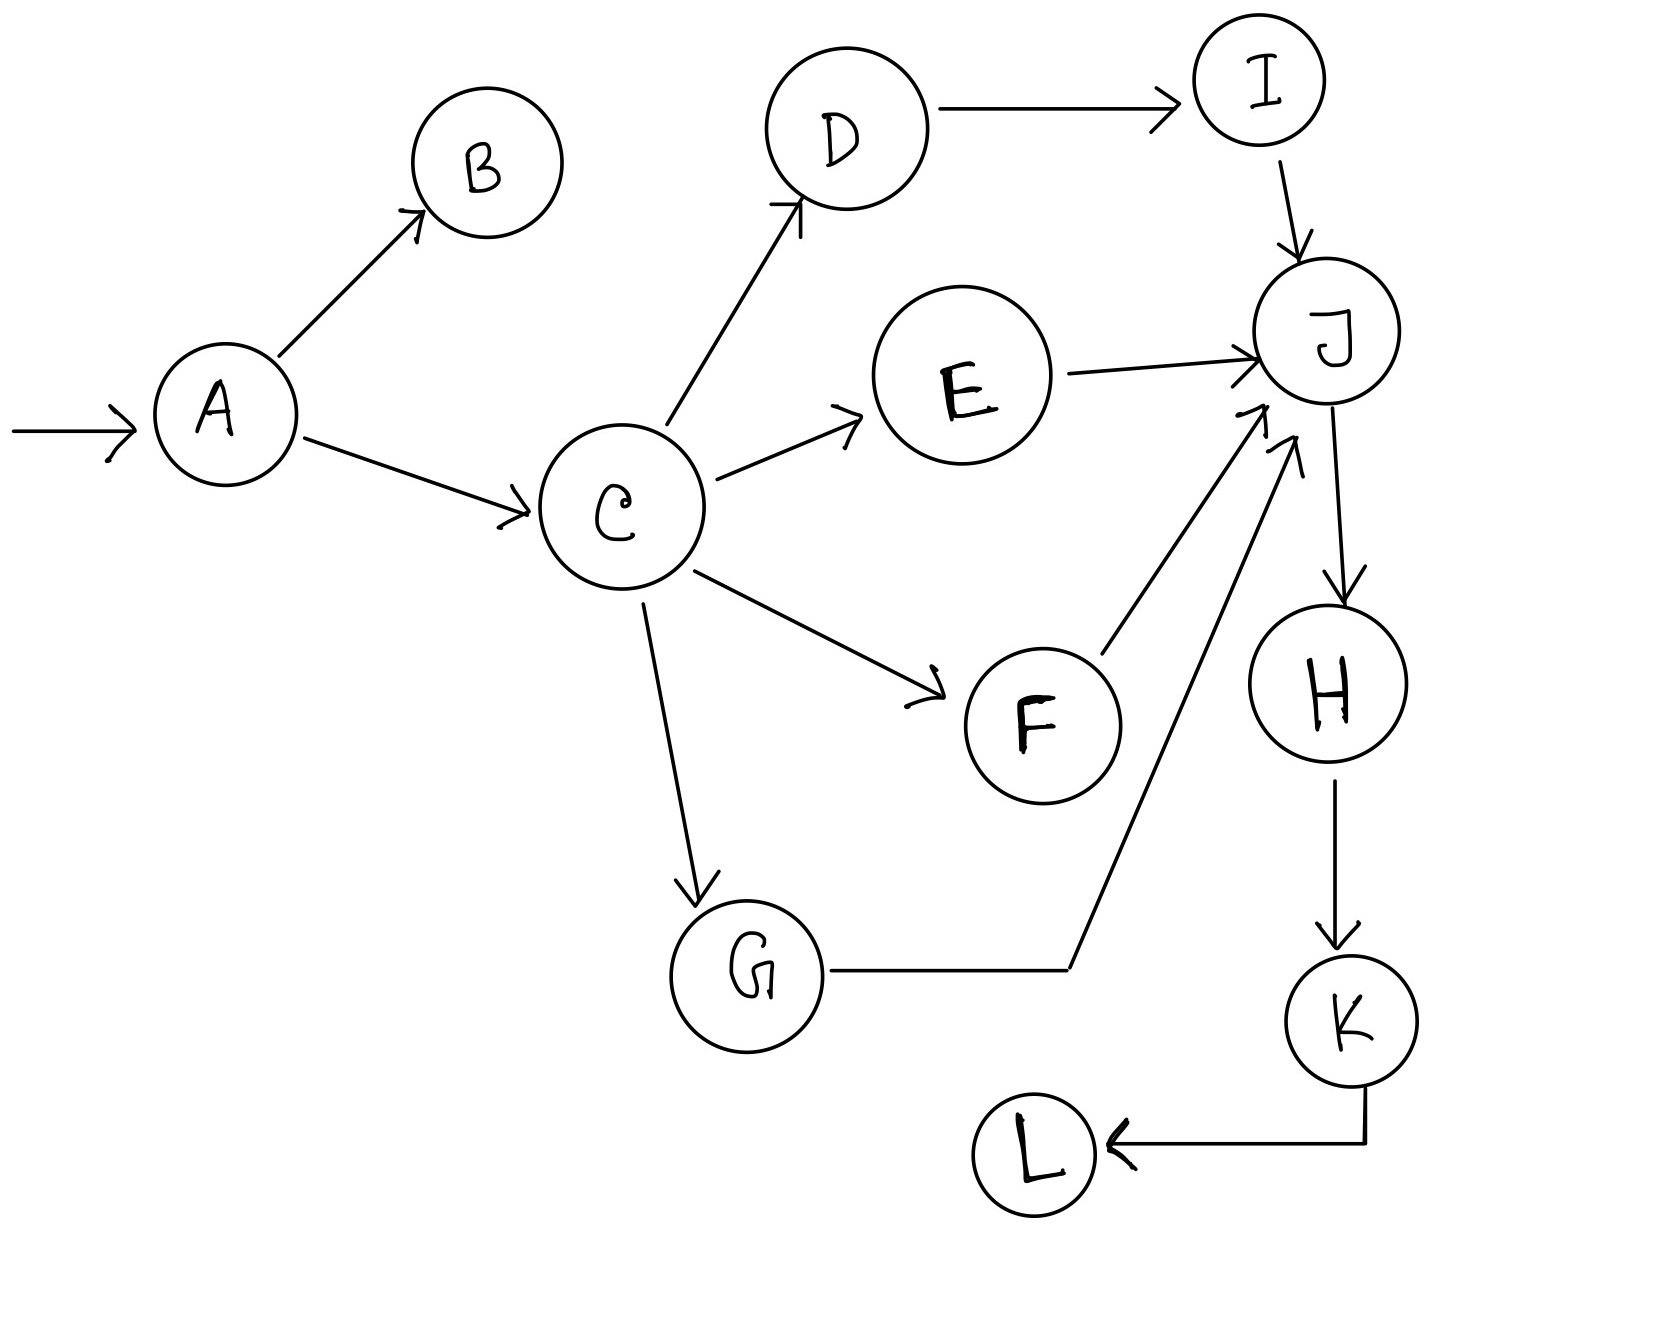
\includegraphics[width=\textwidth, height=3in]{AON}
	\caption{AON network graph}
	\label{fig:aon}
\end{figure} 

\end{spacing}